\clearpage
\makeatletter
\efloat@restorefloats
\makeatother


\begin{appendix}
\section{}
\hypertarget{simulation}{%
\subsection{Simulation}\label{simulation}}

A possible concern with these results -- substantially better predictive
performance for bi-modal mixture models -- is that, in principle, as the
mixture model has more parameters it might always lead to a better fit.
We addressed this concern before by using cross-validation techniques
for model comparison which is preventing overfitting models. To address
this concern we repeated a comparison for a uni-modal model and a
bi-modal mixture model for two sets of simulated data that were
simulated either with a uni-modal or bi-modal process at heart. In other
words, this allows us to test the predictive performance of our models
in a context where we know the true underlying data generating process
-- uni-modal vs bi-modal -- and we can test whether these models can
successfully uncover the true parameter value.

In particular, the first data set was simulated using a bi-modal mixture
model with two mixture components similar to the process described above
(equations in \ref{eq:bimodcon} and \ref{eq:bimoduncon}). This process
and the corresponding Bayesian model is summarised in equation
\ref{eq:simmog}.

\begin{equation}
\begin{aligned}
(\#eq:simmog)
\text{y} \sim\text{ } & \theta \cdot \text{logN}(\beta + \delta, \sigma^2_1) +\\
& (1 - \theta) \cdot \text{logN}(\beta, \sigma^2_2)\\
\text{constraint: } & \delta, \sigma_\text{2}^2, \sigma_\text{1}^2>0\\
        & \sigma_{1}^2 > \sigma_{2}^2
\end{aligned}
\end{equation}

This model is largely identical to the models before but reduced to its
main parameters (but not mixed effects for participants). The model
includes two log-normal distributions with a mixing proportion
\(\theta\) of which the distribution of shorter values has a mean of
\(\beta\) and a standard deviation \(\sigma^2_2\); the second
distribution of longer values is constrained to have a mean that is
larger by a factor of \(\delta\) and has a larger standard deviation
\(\sigma^2_1\).

The second data set was generated with a uni-modal log-Gaussian process.
The model and its corresponding Bayesian model is summarised in equation
\ref{eq:simuv}.

\begin{equation}
\begin{aligned}
(\#eq:simuv)
\text{y} \sim\text{ }& \text{logN}(\beta, \sigma^2)\\
\text{constraint: } & \sigma^2>0
\end{aligned}
\end{equation}

Again, this model is a simplified version of the uni-modal models used
in the main analysis. The model assumes a log-Gaussian distribution with
a mean parameter \(\beta\) and a standard deviation \(\sigma^2\).

The parameter values used for each of the two data simulations can be
found in Table \ref{tab:simparam}. The simulated data are visualised in
Figure \ref{fig:simdata}. Parameter values were chosen so that the
simulated data are roughly similarly distributed to keystroke
transitions.

\begin{figure}

{\centering 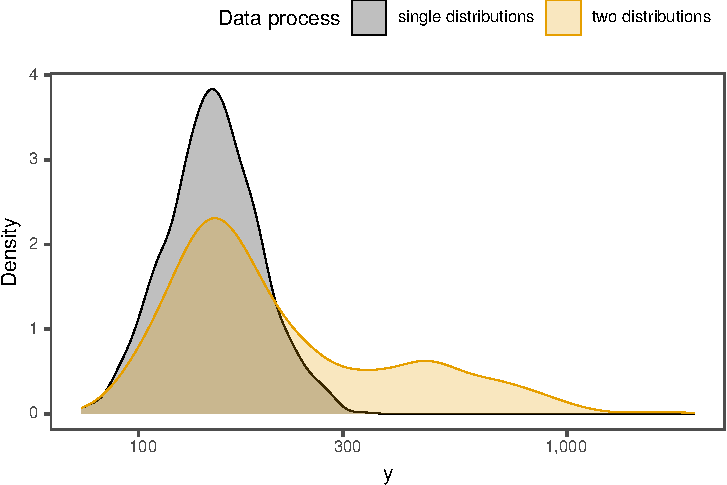
\includegraphics{manuscript_files/figure-latex/simdata-1} 

}

\caption{Data simulated with a bi-modal (grey) and a uni-modal (yellow) random data generating process. The x-axis showing the outcome y was log-scaled for visability.}(\#fig:simdata)
\end{figure}

For each of these two data sets we simulated 1,000 observations. We run
2 models -- a bi-modal mixture model and a uni-modal model -- each for
both data sets. Models were run with 3 chains, with each 6,000
iterations of which 3,000 were warmup. Estimates with 95\% probability
intervals are shown in Table \ref{tab:simparam}. The parameters are
shown by type of data generating process along with the true parameter
values. Parameter value estimates are shown by type of Bayesian model.
The results show that either of the two Bayesian models succesfully
uncovered the model parameters of the data with its corresponding data
generating process, as shown in Table \ref{tab:simparam}, but less so
when the model was applied to data generated with the incorrect
underlying process. Particularly the mixing proportion \(\theta\) and
the slowdown parameter \(\delta\) were not uncovered at all by they
uni-modal model.

\begin{table}[tbp]

\begin{center}
\begin{threeparttable}

\caption{\label{tab:simparam}Uncovered parameter estimates with 95\% probability interval (PI) and true parameter values for each simulated data set and by model and their respective parameters.}

\begin{tabular}{lrr}
\toprule
 & \multicolumn{2}{c}{Estimate with 95\% PI} \\
\cmidrule(r){2-3}
Parameter with true value & \multicolumn{1}{c}{Bi-modal model} & \multicolumn{1}{c}{Uni-modal model}\\
\midrule
Bi-modal data &  & \\
\ \ \ $\beta = 5$ & 5.02 [4.99, 5.04] & 4.93 [4.76, 5.01]\\
\ \ \ $\delta = 1$ & 1.04 [0.92, 1.14] & 0.13 [0.01, 0.3]\\
\ \ \ $\theta = .35$ & .33 [.28, .39] & .54 [.11, .92]\\
\ \ \ $\sigma^2_1 = 0.25$ & 0.25 [0.23, 0.27] & 0.22 [0.16, 0.25]\\
\ \ \ $\sigma^2_2 = 0.5$ & 0.49 [0.42, 0.57] & 0.25 [0.22, 0.3]\\
Uni-modal data &  & \\
\ \ \ $\beta = 5$ & 5.35 [5.32, 5.39] & 5 [4.99, 5.02]\\
\ \ \ $\sigma = 0.25$ & 0.6 [0.57, 0.63] & 0.25 [0.24, 0.26]\\
\bottomrule
\end{tabular}

\end{threeparttable}
\end{center}

\end{table}

We used LOO-CV to compare the predictive performance of the two models
for each data generating process. The model comparisons can be found for
each data generating process in Table \ref{tab:loossim}. The results
rule out the possibility that the mixture model does always lead to
higher predictive performance. Indeed, the mixture model showed a
slightly lower predictive performance for the data that were generated
with a uni-modal process. However, for the data generated with a
bi-modal process, the mixture model shows a substantially higher
predictive performance. In fact, the ratio of \(\Delta\widehat{elpd}\)
and its standard error, as metric for the strength of evidence (Sivula
et al., 2020), shows that the mixture model performs 11.6 times better
than the uni-modal model. In comparison, for the uni-modal data, the
uni-modal model performs only 0.77 times better than the bi-modal
mixture model. Thus, as the difference \(\Delta\widehat{elpd}\) between
the model is negligible, the uni-modal is preferred by the law of
parsimony.

\begin{table}[tbp]

\begin{center}
\begin{threeparttable}

\caption{\label{tab:loossim}Model comparisons by data set. The top row shows the models with the highest predictive performance for each data generating process. Standard error is shown in parentheses.}

\begin{tabular}{lrr}
\toprule
Model & \multicolumn{1}{c}{$\Delta\widehat{elpd}$} & \multicolumn{1}{c}{$\widehat{elpd}$}\\
\midrule
Data: Bi-modal mixture process &  & \\
\ \ \ Bi-modal mixture model & -- & -6,068 (41)\\
\ \ \ Uni-modal model & -191.3 (16.5) & -6,259 (38)\\
Data: Uni-modal process &  & \\
\ \ \ Uni-modal model & -- & -5,030 (24)\\
\ \ \ Bi-modal mixture model & -0.5 (0.7) & -5,030 (24)\\
\bottomrule
\addlinespace
\end{tabular}

\begin{tablenotes}[para]
\normalsize{\textit{Note.} $\widehat{elpd}$ = predictive performance indicated as expected log pointwise predictive density; $\Delta\widehat{elpd}$ = difference in predictive performance relative to the model with the highest predictive performance in the top row.}
\end{tablenotes}

\end{threeparttable}
\end{center}

\end{table}
\end{appendix}
